\documentclass[french, utf8]{article}
\usepackage[utf8]{inputenc}
\usepackage[T1]{fontenc}
\usepackage[french]{babel}
\usepackage[parfill]{parskip}
\usepackage{amsmath}
\usepackage{amssymb}
\usepackage{amsfonts}
\usepackage{graphicx}
\usepackage{subfigure}
\usepackage[font={small}]{caption}
\usepackage{float}
\usepackage{listingsutf8}
\usepackage{fullpage}
\usepackage[nochapter]{vhistory}
\usepackage{hyperref}
\usepackage{titlesec}
\usepackage{xcolor}
\usepackage{verbatim}
\usepackage{graphicx}
\usepackage{subcaption}
\usepackage{comment}
%\usepackage[export]{adjustbox}
\usepackage{adjustbox}


\newcommand*{\MyIncludeGraphicsMaxSize}[2][]{%
\begin{adjustbox}{max size={\textwidth}{\textheight}}
    \includegraphics[#1]{#2}%
\end{adjustbox}
}

% -----------------------------------------------------
% -----------------------------------------------------
% -----------------------------------------------------

\hypersetup{
%couleurs des liens cliquable changée pour une meilleur lisibilité
    colorlinks=true,
    linkcolor=blue,
    filecolor=magenta,
    urlcolor=cyan,
    pdfpagemode=FullScreen,
    }

\title{Quoridor Software Requirement Document \\
\large INFO-F209 - Projet d'informatique 2}
\author{Anton Romanova, Mohammad Secundar, Esteban Aguililla Klein, \\
Vlad Moruntale, Mathieu Van Den Bremt, Nabil Abdellaoui, \\
Ayman Boulaich, Noé Bourgeois, Mamadou Balde
}
\date{Decembre 2021}

\begin{document}
\maketitle
\tableofcontents
\newpage


% -----------------------------------------------------
% -----------------------------------------------------
% -----------------------------------------------------
\section{Introduction}
% -----------------------------------------------------
\subsection{But}
Faire un portage du jeu de plateau classique multijoueur Quoridor\footnote{les règles détaillées peuvent être consultées dans la section \nameref{sec:Annexes}} par le biais d'une interface client-serveur et l'ajout de fonctionnalités sociales modernes.
\\ \\
Pour que la partie se termine, dans le mode classique, il suffit d'atteindre le côté opposé du plateau tout en empêchant l'adversaire de faire de même à l'aide de murs plaçables.    %TODO: dans le mode X, il faut Y
\\ \\
Concernant les fonctionnalités sociales, il est possible de gérer une liste d'amis, discuter avec ces derniers, créer une partie privée et consulter un classement des joueurs.
\\ \\
De par sa nature simple, le jeu se veut tout public malgré ses fonctionnalités sociales non modérées.  %ressemblance avec réseau social donc >13 ans min ???

% -----------------------------------------------------
\subsection{Glossaire}

\begin{center}
\begin{tabular}{p{5cm} p{10cm}}
    \textbf{Client} : & Application client \\
    \textbf{Game/Jeu} : & Partie de jeu Quoridor \\
    \textbf{TLS} : & Transport Layer Security \\
    \textbf{Bibliothèque header-only} : & Une bibliothèque composée uniquement de fichiers headers. Les définitions des fonctions, classes et macros sont donc dans des fichiers headers. \\
    \textbf{Utilisateur} : & Un individu possédant les identifiants pour se connecter à un compte existant dans la base de données ou ayant l'intention d'en créer un \\
    \textbf{Joueur} : & Individu ou machine qui participe à un jeu Quoridor\\

\end{tabular}\\
\end{center}
% -----------------------------------------------------
% AJOUTEZ TOUS VOS CHANGEMENTS ICI
\subsection{Historique du document}

\begin{versionhistory}
\vhEntry{0.1.31}{05.03.22}{Bourgeois Noé }{ajout de la fonction MyIncludeGraphicsMaxSize et du diagramme de sequence de création de compte et mise à jour du diagramme de sequence de connexion}
\vhEntry{0.1.30}{04.03.22}{Mathieu Van Den Bremt }{Modification des tableau des USe Case et modification de certains newpage}
\vhEntry{0.1.29}{04.03.22}{Ismaël Secundar }{Ajout des aperçu des menus et modification du use case du menu}
\vhEntry{0.1.28}{01.03.22}{Bourgeois Noé }{division du Diagramme de séquence de connexion en 3 sous-sections et integration avec le texte}
\vhEntry{0.1.27}{27.02.22}{Boulaich Ayman }{Réaménagement des différents diagrammes dans leurs contextes dans le srd}
\vhEntry{0.1.26}{25.02.22}{Boulaich Ayman }{Ajout protocole}
\vhEntry{0.1.25}{25.02.22}{Boulaich Ayman }{Ajout des librairies}
\vhEntry{0.1.24}{23.02.22}{Anton Romanova \& Ismaël Secundar \& Abdellaoui Nabil }{Description du menu actuel et aperçu du menu principal}
\vhEntry{0.1.24}{23.02.22}{Anton Romanova \& Ismaël Secundar \& Abdellaoui Nabil }{Description du menu actuel et aperçu du menu principal}
\vhEntry{0.1.23}{13.12.21}{Anton Romanova \& Bourgeois Noé }{correction du Diagramme de séquence de connexion}
\vhEntry{0.1.22}{13.12.21}{Anton Romanova \& Ismaël Secundar \& Mathieu Van Den Bremt}{Ajout du diagramme pseudo-UML de l'API + section API}
\vhEntry{0.1.21}{10.12.21}{Aguililla Klein Esteban \& Moruntale Vlad}{Ajout du diagramme de séquence expliquant le déroulement d'un tour}
\vhEntry{0.1.20}{10.12.21}{Aguililla Klein Esteban \& Moruntale Vlad}{Ajout de la description des modes de jeux}
\vhEntry{0.1.19}{9.12.21}{Romanova Anton, Ismaël Secundar}{ Relecture \& corrections orthographiques et grammaticales}
\vhEntry{0.1.18}{8.12.21}{ Mathieu Van Den Bremt, Abdellaoui Nabil }{Ajout du diagramme des classes pour les menus}
\vhEntry{0.1.17}{28.11.21}{Bourgeois Noé }{Ajout du diagramme de séquence de connexion}
\vhEntry{0.1.17}{28.11.21}{Bourgeois Noé }{ typos, amélioration du calcul d'actualisation du classement, correction use case de gestion de compte}
\vhEntry{0.1.16}{24.11.21}{Anton Romanova}{Ajout de Mamadou Balde dans la liste des auteurs + fix stylistiques mineurs}
\vhEntry{0.1.15}{24.11.21}{Abdellaoui Nabil }{Cas de disqualification et sauvegarde de partie}
\vhEntry{0.1.14}{24.11.21}{Boulaich Ayman }{Gestion de partie et connexion}
\vhEntry{0.1.13}{24.11.21}{Bourgeois Noé }{Base De Données}
\vhEntry{0.1.12}{23.11.21}{Bourgeois Noé }{Logging}
\vhEntry{0.1.11}{21.11.21}{Romanova Anton, Ismaël Secundar}{Section ``Style de programmation’’ et ``Internationalisation et Localisation’’}
\vhEntry{0.1.10}{21.11.21}{Romanova Anton, Ismaël Secundar}{Ajout de la sous-section 3.2.3 (Concurrence)}
\vhEntry{0.1.9}{21.11.21}{Bourgeois Noé }{Actualisation du classement, colorisation du texte, hyperreferences, use case de gestion de compte}
\vhEntry{0.1.8}{20.11.21}{Bourgeois Noé }{Lancement, enregistrement, créer une partie, rejoindre une partie}
\vhEntry{0.1.7}{20.11.21}{Mathieu Van Den Bremt \& Nabil Abdellaoui}{Modification des UseCase et amélioration divers pour User requirements}
\vhEntry{0.1.6}{19.11.21}{Romanova Anton, Ismaël Secundar}{Brouillon pour besoins non-fonctionnels des besoins système}
\vhEntry{0.1.5}{19.11.21}{Aguililla Klein Esteban \& Moruntale Vlad}{Ajout du but et d'un annexe}
\vhEntry{0.1.4}{19.11.21}{Mathieu Van Den Bremt }{Tableau Use Case}
\vhEntry{0.1.3}{19.11.21}{Boulaich Ayman }{Sous section des besoins fonctionnels du système et début }
  \vhEntry{0.1.2}{18.11.21}{Anton Romanova}{Ajout de la section "Annexes" et "Design"}
   \vhEntry{0.1.1}{17.11.21}{Mathieu Van Den Bremt \& Nabil Abdellaoui}{Début Besoin d'utilisateur + diagrammes Use Case}
  \vhEntry{0.1}{16.11.21}{Anton Romanova}{Structure générale}
\end{versionhistory}

% -----------------------------------------------------
% -----------------------------------------------------
% -----------------------------------------------------
\newpage
\section{Besoin d'utilisateur}
% -----------------------------------------------------

\subsection{Besoins/Exigences fonctionnelles}
%Connexion
%Démarrer une partie
%Actions durant une partie
%Visualisation classement

\subsubsection{Menu de bienvenu}
\label{sec:Menu de bienvenu}
En démarrant le jeu, un menu de bienvenu apparaîtra. Si l'utilisateur n'a pas de compte il aura la possibilité d'en créer un.

\begin{figure}[ht]
     \centering
    %\includegraphics[width=70mm,scale=0.1]{Image/SystemUC.PNG}
    \includegraphics[width=50mm,scale=0.1]{Image/Welcome.png}
\caption{Aperçu du menu de bienvenu}
\end{figure}

\subsubsection{Menu principal}

\label{sec:Menu principal}

Une fois la connexion faite, l'utilisateur basculera sur le menu d'accueil. Il aura plusieurs choix. Il pourra notamment lancer une partie, ajouter un(e) ami(e) et échanger des messages avec, consulter la liste des meilleurs joueurs et leurs score. Dans le cas où l'utilisateur a besoin d'aide, il pourra accéder à un menu qui va l'aiguiller.
De plus, si un utilisateur se déconnecte de son compte un autre peut se connecter avec un autre compte. Chacun aura évidemment son compte propre à lui.

L'utilisateur pourra naviguer entre les différentes options grâce aux Touches directionnelles du clavier.  \newline

\begin{figure}[ht]

     \centering
    %\includegraphics[width=70mm,scale=0.1]{Image/SystemUC.PNG}
    \includegraphics[width=50mm,scale=0.1]{Image/Accueil.png}
\caption{Aperçu du menu principal}
\end{figure}
%%%%%%%%%%%%%%%%%%%%%%%%%%%%%%%%%%%%%%%%%%%%%%%%%%%%%%%%%%%%%%%%%%%%%%%%%%%%%%
%%%%%%%%%%%%%% A COMPLETER
L'utilisateur pourra configurer sa partie en modifiant plusieurs paramètres. Il devra indiquer le nombre de participants qui seront dans la partie. Ils pourront être 2 ou 4. Par la suite, il devra indiquer quels utilisateurs, parmi la liste d'amis, pourront rejoindre la partie. Les joueurs invités devront évidemment confirmer leur participation. Une fois que tout ceci est fait, les joueurs attendront que leurs adversaires rejoignent la partie avant de commencer à jouer. \newline

Si le cours d'une partie a été précédemment sauvegardé, l'utilisateur pourra la reprendre là où elle s'était arrêtée à condition que tous les autres participants soient présents pour continuer.

Si il le désire, l'utilisateur pourra aussi demander de l'aide, l'application affichera le fonctionnement du jeu et les différentes fonctionnalités de cette dernière.
%%%%%%%%%%%%%%%%%%%%%%%%%%%%%%%%%%%%%%%%%%%%%%%%%%%%%%%%%%%%%%%%%%%%%%%%%%%%%%



%\newline

\begin{figure}[ht]
     \centering
    %\includegraphics[width=70mm,scale=0.1]{Image/SystemUC.PNG}
    \includegraphics[width=130mm,scale=0.1]{Image/MainScreenUC.jpg}
\caption{Diagramme Use Case Des Menus. On peut y voir toute les actions possible depuis le menu principal.}
\end{figure}


\begin{center}
\begin{tabular}{|m{3cm}|m{3cm}|m{3cm}|m{3cm}|m{3cm}|}
\hline  Use Case & Pré condition      &  Post condition  & Cas général & Cas exceptionnels\\
\hline Play & Néant & En fin de partie les résultat sont mis à jour dans le Ranking & Le programme lance la configuration d'une partie puis lance celle-ci après avoir lancé l'invitation d'un joueur & L'invité refuse l'invitation, l'utilisateur est notifié que l'invité a refusé l'invitation \\
\hline Chat & Néant & L'utilisateur voit sa liste d'ami(e)s & L'utilisateur cible l'ami avec qui il veut parler & L'utilisateur n'est pas ami avec la cible, il peut chercher l'ami en l'ajoutant \\
\hline Ranking & Un classement existe  & L'utilisateur voit le classement & Le programme montre le classement des meilleurs joueurs & Néant \\
\hline Help & L'utilisateur a besoin d'aide  &  Néant & Une explication brève du jeu s'affiche & Néant \\
\hline Send message to friend & l'utilisateur cible existe & Le message est envoyé & Le programme envoie un message écrit par l'utilisateur à une personne de la liste d'amis de celui-ci & l'utilisateur s'envoie un message à lui-même, une erreur s'affiche \\
\hline Search in friend list & l'utilisateur cherche un ami & Néant & L'utilisateur trouve l'ami qu'il cherchait dans sa liste d'amis & Néant \\
\hline Search friend & l'utilisateur cherche l'ami qui doit être ajouté & L'utilisateur ajoute l'ami & Le programme sauvegarde le contact du nouvel ami dans la liste & Néant \\
\hline Invite Friend to Game & L'ami invité doit faire partie de la liste d'ami & L'ami rejoint la partie & Le programme permet à l'utilisateur d'inviter un ami à jouer avec lui & Si l'ami ciblé refuse l'invitation, le programme notifie l'utilisateur que l'ami ciblé a refusé \\
\hline Join Game & Un autre utilisateur a invité l'utilisateur & L'utilisateur rejoint la partie & Le programme invite l'utilisateur à rejoindre une partie & Si l'utilisateur refuse alors le programme envoie un message à l'utilisateur qui a envoyé l'invitation \\
\hline Play Game & Néant & En fin de partie les résultat sont mis à jour dans le classement & Le programme démarre la partie & Si la partie est quittée en cours de jeu, alors le classement n'est pas mis à jour \\
\hline Logout  & Néant & Le programme retourne à l'écran de connexion & Le programme déconnecte le joueur & Néant \\

\hline
\end{tabular}\\
\end{center}
\label{sec:MenuPrincipalUser}
Diagramme de classe des menus:
\begin{figure}[ht]
\centering
    \includegraphics[width=170mm,scale=0.1]{Image/mvc_menu.PNG}
\end{figure}

Le diagramme ci-dessus représente tout le fonctionnement orienté MVC des menus. D'une part il y a les contrôleurs qui interagissent avec l'utilisateur et qui attendent une entrée de la part de ces derniers, et d'autre part il y a les vues qui, comme leurs noms l'indiquent, sont la partie visuelle des menus. \newline



\subsubsection{Durant une partie}
Quand c'est son tour, le joueur doit pouvoir effectuer une action, déplacer un pion ou mettre un mur. Cette action est représentée comme un message envoyé à l'application qui agira sur lui-même en conséquence.
En plein duel, l'un des joueurs peut proposer au reste des participants de mettre le jeu en pause et de sauvegarder la partie en cours pour pouvoir la continuer plus tard. Les joueurs peuvent aussi déclarer forfait et donc se retirer. \newline
Si l'un des joueurs se déconnecte sans proposer de sauvegarder la partie, il est considéré comme disqualifié, la partie est interrompue et son opposant ressort gagnant. Il en est de même pour une partie à 4 sauf qu'aucun gagnant n'est déterminé.
%mettre une référence au diagramme de séquence de déroulement de la partie
\newline

\begin{figure}[ht]
     \centering
    %\includegraphics[width=70mm,scale=0.1]{Image/GameUC.PNG}
    \includegraphics[width=110mm,scale=0.1]{Image/GameUC.png}
\caption{Diagramme Use Case d'une partie de jeu}
\end{figure}
%ligne vide tableau : \hline .  & . & . & . &. \\
\begin{center}
\begin{tabular}{|m{3cm}|m{3cm}|m{3cm}|m{3cm}|m{3cm}|}
\hline  Use Case & Pré condition      &  Post condition  & Cas général & Cas exceptionnels\\
\hline Play Game & L'utilisateur à lancer et configurer une partie et il y a un nombre requis de Joueur & A la fin de la partie on retourne sur l'écran principal & Le programme lance le jeu Quoridor et demande tour par tour, quel actions les joueur veulent faire & Si un joueur quitte en cours de partie un message est envoyé à l'adversaire  \\
\hline Move pawn  & Le pion peut être déplacé comme le veut l'utilisateur & Le plateau est modifié avec la nouvelle position du pion & Le programme déplace le pion & Néant \\
\hline
\end{tabular}\\
\end{center}
\begin{center}
\begin{tabular}{|m{3cm}|m{3cm}|m{3cm}|m{3cm}|m{3cm}|}
\hline Place Wall  & L'emplacement désigné pour le mur est libre et ne bloque pas entièrement un pion & Le plateau est modifié avec le nouveau mur & Le programme place un mur dans la position choisie & Néant \\
\hline Pause Game  & Néant & Le jeu est mis en pause, sauvegardé et ensuite terminé & Le programme demande à l'adversaire si celui-ci accepte de mettre en pause le jeu & Néant \\
\hline Save  & Le jeu a été mis en pause sur l'accord des deux joueurs & La partie est sauvegardée & Le programme sauvegarde la partie tel qu'elle est & Si le programme n'a pas réussi à sauvegarder les données, alors celui-ci envoie un message d'erreur \\
\hline Forfeit  & Néant & La partie est terminée sur une victoire adverse & Le programme termine la partie & Néant \\
\hline
\end{tabular}\\
\end{center}

\subsubsection{Mode de jeux}
\
L'utilisateur peut choisir un mode de jeux différent au mode classique parmi les modes suivants.
\paragraph{Murs aléatoires}

Des murs apparaissent de façon aléatoire\footnote{les murs ne pourront pas bloquer totalement le chemin d'un joueur vers son objectif} sur le plateau.
\paragraph{Humain contre ordinateur}

L'adversaire est contrôlé par l'ordinateur. Ce dernier est capable des mêmes actions qu'un joueur normal.

% -----------------------------------------------------

\subsubsection{Légalité}
L'utilisateur peut supprimer son compte selon le GDPR.

\subsubsection{Messagerie}
L'utilisateur pourra voir la date et l'heure d'envoi d'un message.

\subsection{Exigences non-fonctionnelles}
\subsubsection{Inscription et connexion}
L'utilisateur doit être capable de présenter un nom de compte ainsi qu'un mot de passe au démarrage du jeu pour pouvoir se connecter et accéder à son menu principal. Si il n'a pas de compte ou si il désire en recréer un, il lui est possible d'en créer un nouveau. Pour la création d'un compte, aucun mail n'est nécessaire à introduire, l'utilisateur doit juste présenter un nouveau pseudonyme accompagné d'un mot de passe pour terminer le processus de création. \newline


\begin{figure}[ht]
     \centering
    %\includegraphics[width=70mm,scale=0.1]{Image/SystemUC.PNG}
    \includegraphics[width=100mm,scale=0.1]{Image/ConnectionUC.PNG}
\caption{Diagramme Use Case pour la connexion}
\end{figure}
\begin{center}
\begin{tabular}{|m{3cm}|m{3cm}|m{3cm}|m{3cm}|m{3cm}|}
\hline  Use Case & Pré condition      &  Post condition  & Cas général & Cas exceptionnels\\
\hline Register& l'utilisateur n'a pas encore un compte & On enregistre le nouveau compte & Le programme demande un nom et un mot de passe & Si le nom est déjà utilisé alors on envoie une erreur  \\
\hline Connect  & L'utilisateur a déjà un compte & L'utilisateur rentre dans le programme & Le programme vérifie les informations données par le client ensuite, il lui permet de continuer sur le programme & Si les informations sont incorrectes, alors on envoie une erreur \\

\hline
\end{tabular}\\
\end{center}

\newpage
\subsubsection{Commande}
L'utilisateur devra entrer une commande pour chaque action qu'il effectuera.
Par exemple les commandes en cours de jeu seront:\\
Pour déplacer un pion: "case de départ">"case d'arrivée"\\
Pour mettre un mur : "première case">"deuxième case">"Direction du mur"
\begin{figure}[ht]
     \centering
    %\includegraphics[width=70mm,scale=0.1]{Image/SystemUC.PNG}
    \includegraphics[width=100mm,scale=0.1]{Image/mouvement_en_terminal.png}
    \caption{Exemple de mouvement lors d'une partie}
\end{figure}

\subsubsection{Déconnexion en partie}
Dans le cas d'une déconnexion durant une partie, le jeu est interrompu et tout les joueurs sont renvoyés au menu principal.

% -----------------------------------------------------
% -----------------------------------------------------
% -----------------------------------------------------
\section{Besoins du système}

% -----------------------------------------------------
\subsection{Besoins fonctionnels}
\begin{comment}
\subsubsection{Lancement}
\label{sec:Lancement}
Le programme, à son lancement,
affiche une fenêtre d'accueil contenant le titre du jeu et demande à l’utilisateur d'entrer :
\\un pseudo
\\un mot de passe

\MyIncludeGraphicsMaxSize{Image/connexion-sequence-shrodinger-user.png}

%Il peut ensuite
%\\soit créer un nouveau compte,
%\\soit se connecter avec un compte déjà %enregistré dans une base de
%donnée.

\end{comment}

\subsubsection{Enregistrement}
\label{sec:Enregistrement}
%TOTP?
Conditions:
\newline
- Le pseudo n'est pas présent dans la Base De Donnée et contient:
\begin{itemize}
\item uniquement des caractères alphanumériques + "\_" + "-"
\item un nombre de caractères entre 3 et 25
\end{itemize}

- Le mot de passe contient:
\begin{itemize}
\item plus de 8 caractères
\item 4 caractères spéciaux
\end{itemize}

Si les conditions sont respectées, le nom d'utilisateur et le mot de passe sont enregistrés dans
la base de données et la fenêtre du
\nameref{sec:MenuPrincipalSystem}
 apparaît.

\begin{comment}
L'utilisateur devra créer un compte, et ainsi enregistrer le compte dans la base de données. Lorsque l'utilisateur entre un pseudo , le programme cherchera celui-ci dans la base de données et avertira l'utilisateur si son compte n'existe pas.
\end{comment}

\MyIncludeGraphicsMaxSize{Image/account-creation-sequence-diagram.png}

\newpage
\subsubsection{Connexion}
\label{sec:Connexion}
Conditions:

L'utilisateur possède un compte:
\newline
Si le pseudo est trouvé et que le mot de passe entré par le joueur correspond alors l'utilisateur sera connecté.
Dans le cas contraire,l'utilisateur est informé par le programme que son mot de passe ne correspond pas au pseudo inscrit.Le programme donnera alors à l'utilisateur la possibilité de retrouver son mot de passe via la réponse à une question secrète stockée dans la base de données lors de l'enregistrement du compte :

\MyIncludeGraphicsMaxSize{Image/login-sequence-diagram.png}

\newpage
\subsubsection{Menu principal}
\label{sec:MenuPrincipalSystem}

Use case: \nameref{sec:MenuPrincipalUser}

\begin{comment}

\subsubsection{Gestion du compte}
\label{sec:GestionDeCompte}
Le système gérera les modifications de l'utilisateur au niveau du compte lorsqu'il est connecté via ce dernier au programme. Le système doit par conséquent mettre a jour la base de données lors des différents changement que peut faire l'utilisateur tels que changer son nom d'utilisateur, son mot de passe, ajouter une description.

Le diagramme de séquence ci-dessous représente les appels API lors de l'exécution de certaines actions de la part de l'utilisateur .
\newpage
\begin{figure}[ht]
\centering
    \includegraphics[width=\textwidth,height=160mm,keepaspectratio]{Image/AccountManagementWithAPISequenceDiaram.png}
\end{figure}

\newline
%Description dans le use case
\begin{figure}[ht]
    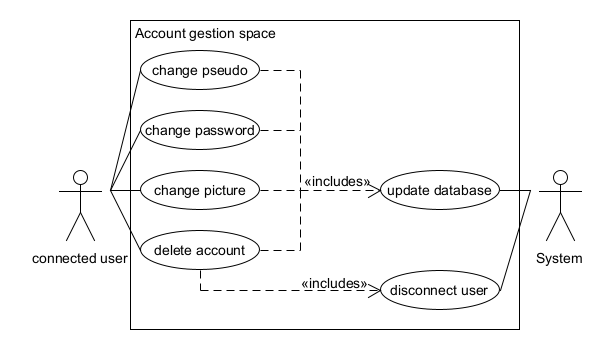
\includegraphics[width=110mm,scale=0.1]{Image/AccountGestionUC.png}
   \caption{Diagramme Use Case Besoin système}
\end{figure}

\begin{center}
\begin{tabular}{|m{3cm}|m{3cm}|m{3cm}|m{3cm}|m{3cm}|}
\hline  Use Case & Pré condition      &  Post condition  & Cas général & Cas exceptionnels\\

\hline Change Pseudo  & conditions d'\nameref{sec:Enregistrement} du pseudo & Le nouveau pseudo est affiché à la place de l'ancien, le nombre de comptes dans la base de données n'a pas changé & Le programme remplace dans la base de données l'ancien pseudo par le nouveau & Néant \\
\hline Change Password  & conditions d'\nameref{sec:Enregistrement} du mot de passe & L'ancien mot de passe n'est plus valide & Le programme remplace dans la base de données l'ancien mot de passe par le nouveau & Néant \\
\hline Change Bio  & Néant & La nouvelle biographie est affiché avec le pseudo de l'utilisateur  & Le programme remplace dans la Base de données l'ancienne biographie par la nouvelle & Néant \\
\hline Delete Account  & Néant &  Le programme déconnecte l'utilisateur  & Le programme supprime dans la base de données toutes les données liées au pseudo du joueur & Néant \\
\hline
\end{tabular}\\
\end{center}
\end{comment}

\subsubsection{Configuration de partie}
\paragraph{Création de partie}
\label{sec:CréationDePartie}
Si l’utilisateur sélectionne
"new game",
une fenêtre de configuration de jeu apparaît contenant les paramètres par défaut:
\item- la taille du plateau: 9
    %-le nombre de pions\\
\item- l'apparition aléatoire de murs sur le plateau: "on" (switch sur GUI)
\item- le mode de jeu
\item- le ou les autre(s) joueur(s):
\item---  un ou des humain(s) qui ont rejoint
\item- l'invitation d'autres joueurs humains sous forme de commande pour ouvrir une fenêtre affichant les joueurs connectés et un espace de recherche
\\L'utilisateur peut les modifier et, à tout moment, démarrer la partie avec les paramètres
affichés

\paragraph{Rejoindre une partie}
\\Si l’utilisateur sélectionne
"join", une liste des joueurs créant une partie apparaît.
\\Il peut en sélectionner une pour la rejoindre.
\\Si l’utilisateur reçoit une invitation, celle-ci est affichée superposée à la fenêtre actuellement affichée sauf si il est en train de jouer.

\subsubsection{Gestion de partie}
\label{sec:GestionDePartie}
%#TODO
Lorsque le joueur lance la partie le plateau du jeu s'affiche en fonction des options de jeu choisi par les joueurs.le système gère alors les différentes manipulations que peuvent faire les joueurs. le joueur peut mettre pause au jeu et déclarer forfait via des commandes  . le système doit aussi actualiser le plateau lorsque le joueur bouge ou place un mur. Le nombre de murs de chaque joueur est connue par le système et est décrémenté à chaque fois que le joueur place un mur sur le terrain.
%pas sur si c'est le bon endroit où le mettre -Vlad & Esteban
%%\begin{figure}[ht]
%\centering
    %\includegraphics[width=\textwidth,height=170mm,keepaspectratio]{Image/TurnSequenceDiagram.png}
%\end{figure}

Voici le diagramme des séquences d'évènements qui se déroulent durant un tour normal pour le joueur.
On y retrouve la connexion entre le client et le serveur lors d'une action demandée par le joueur.
Diagramme de séquence représentant la création d'un jeu

\begin{figure}[ht]
\centering
    % \includegraphics[width=170mm,scale=0.4]{Image/Client-Server Game Creation Sequence Diagram.png}
    \includegraphics[width=\textwidth,height=170mm,keepaspectratio]{Image/Diagramme de séquence représentant la création d'un jeu.png}
\end{figure}

\subsubsection{Actualisation du classement}
\label{sec:ActualisationDuClassement}

Après une partie, le classement est mis à jour:
\\- Si c'est une égalité, les scores ne changent pas.

- Sinon,
les classements du gagnant et du perdant sont respectivement augmentés et diminués de \\

\[
 \frac{\text{(taille du plateau + nombre de murs) * (score perdant + 1)}}{\text{nombre de tours * score gagnant + 1}}
\]

\\- Le classement d'un joueur ne descend pas sous 0



\subsubsection{Base de données}
\label{sec:BaseDeDonnées}

La base de donnée \href{https://en.wikipedia.org/wiki/SQL}{SQL} contient :
\item- les données correspondant à chaque joueur:
\item--- pseudo (:clé)
\item--- mot de passe % Salted hash + salt
\item--- chemin d'accès vers le fichier de l'image du profil
\item--- classement
\item--- liste d'amis
\item--- liste de conversations
\item--- liste de parties enregistrées

\item--- les conversations
\item- les parties enregistrées
%\\ \item--- la liste des participants
\item- le classement

\subsubsection{Logging}
\label{sec:Logging}
Tout évènement du programme incluant un accès à la base de données est enregistré sous forme ASCII ou binaire dans un log file et consultable par l'administrateur système sous forme ASCII.

\subsubsection{Mode de jeu}
Le système doit adapter les règles du jeu selon le mode de jeu choisi par l'utilisateur.

\subsubsection{Latence}
Toutes les actions doivent passer d’un utilisateur à un autre avec une latence minimale en mettant à jour le plateau le plus rapidement possible et ainsi donner l'illusion que les actions se font instantanément.

\subsubsection{API}
Le programme utilise une REST API pour les communications entre le client et le serveur. L'API qui sera implémentée à l'aide de la bibliothèque Craw. Cette bibliothèque est header-only, ce qui permettra de faciliter la portabilité.
Les appels se font sous forme de requêtes "GET".
L'authentification de l'utilisateur se fait à l'aide d'un token d'accès temporaire régénéré à chaque nouvelle connexion de la part du client.
Les appels API assurent toute la communication client-serveur et permettent entre-autres de garder les parties des adversaires synchronisées, mais aussi avoir un des chats avec d'autres utilisateurs, ou tout simplement consulter les informations sur d'autres joueurs (par exemple, leur biographie).

\begin{figure}[ht]
\centering
    \includegraphics[width=200mm,height=150mm,keepaspectratio]{Image/Quoridor API.png}
\end{figure}
Dans ce diagramme on remarque, est reprensenté chaque connexion au serveur par l'intermédiaire de l'api. Chaque chemin ici présent fonctionne comme une uml

\subsubsection{diagramme de classe Server side}
\begin{figure}[ht]
\centering
    \includegraphics[width=\textwidth,height=170mm,keepaspectratio]{Image/ServerSideClassDiagram.png}
\end{figure}



% -----------------------------------------------------
\subsection{Besoins non-fonctionnels}
Contraintes liées au matériel

\subsubsection{Portabilité}

Le programme doit fonctionner sur Linux. Si possible sans trop de modifications, il devrait également être compatible avec Windows.

\subsubsection{Réseau}

Les clients et le serveur doivent être connectés à un même réseau. Lorsqu'un joueur se déconnecte subitement du serveur, le serveur doit en avertir d'autres serveurs clients qui ont une partie en cours avec le joueur déconnecté.

\subsubsection{Concurrence}

Afin de pouvoir gérer plusieurs connexions, le programme serveur doit s'exécuter en parallèle. Les transactions de la base de données effectuées en concurrence ne peuvent pas violer l'intégrité des données. Le contrôle optimiste de la concurrence sera utilisé, pour améliorer les performances et éviter les deadlocks.

Du côté client, la concurrence doit également être utilisée pour avoir une interface graphique utilisateur (GUI) réactive.

\subsubsection{Sécurité}

Pour que l'envoi de données sensibles à travers internet ne puisse pas être intercepté, la communication devra se faire à l'aide d'un protocole de communication crypté. Un choix évident serait le TLS.

Une session pourra rester active à l'aide d'un access token.
Ce token aura une date d'expiration. Le programme client gardera ce token dans la RAM.
Ainsi, après le redémarrage du programme client, l'utilisateur devra se reconnecter avec son nom d'utilisateur et son mot de passe.


En ce qui concerne le programme serveur, celui-ci gardera un salted hash du mot de passe dans la base de données.

La récupération de mots de passe pourra se faire avec des questions secrètes ou éventuellement avec des mots de passes à usage unique générés à l'aide du standard TOTP (le client pourra, par exemple, les générer avec Google Authenticator ou l'alternative open-source, RavioOTP).


\subsubsection{Fiabilité}

Lorsque le client se déconnecte du serveur au cours d'une partie, l'adversaire doit en être averti.
Après une minute d'attente, le joueur déconnecté est déclaré perdant suite à un abandon.

\subsubsection{Internationalisation et Localisation}

Dans le contexte de ce projet d'année, le programme ne sera pas internationalisé.
Les timestamps (date des messages, création de parties, ... ) seront enregistrés en timestamp unix. Ainsi, les clients se trouvant dans un fuseau horaire différent pourront voir ces timestamps en heure locale


\subsubsection{Légalité}
Le système ne garantit pas le respect du GDPR excepté pour la suppression de compte.

% -----------------------------------------------------

\section{Design et fonctionnement du système}

% -----------------------------------------------------


\subsection{Jeu}
Voir Annexe I

Diagramme de séquence expliquant les interaction client-serveur lorsqu'un joueur joue son tour

% -----------------------------------------------------
% -----------------------------------------------------

\section{Annexes}
\appendix

\label{sec:Annexes}
\section{Style de programmation}

Dans le cadre de ce projet, le style de programmation défini par Google:
\\ \href{https://google.github.io/styleguide/cppguide.html}{https://google.github.io/styleguide/cppguide.html}
\\ voir \href{https://google.github.io/styleguide/cppguide.html#Naming}{Google Naming conventions}
\\doit être utilisé.

En résumé,
\begin{itemize}
	\item L'indentation est de 2 espaces,
	%les noms de variable je pense et pareil pour les autres trucs
	\item Les noms des fichiers en minuscule avec des ``-’’ et des ``\_’’
	\item Les noms des classes, des structs et des méthodes sont en CamelCase et commencent par une majuscule
	\item Les noms des variables sont en minuscules et séparés par des ``\_’’
	\item Les attributs privés terminent par un ``\_’’
	\item les constantes sont en CamelCase et commencent par un k minuscule (ex: kRefreshRate)
\end{itemize}

\section{Règles de base de Quoridor}
Ces dernières peuvent être consultées sur le site de son éditeur Gigamic \\\href{https://www.gigamic.com/files/catalog/products/rules/quoridor-classic-fr.pdf}{https://www.gigamic.com/files/catalog/products/rules/quoridor-classic-fr.pdf}
\section{Librairies}
Dans le cadre de ce projet d'année , les librairies utilisées sont :
\begin{itemize}
    \item ncurses
    \item Algorithm
    \item boost
\end{itemize}

\section{Lancement de jeu}
Pour lancer le jeu il faut utiliser les commandes suivantes sur Ubuntu :
cmake .
cmake --build . --target ClientSide
cmake --build . --target QuoridorServer



\section{Commentaires sur les diagrammes}
Les diagrammes séquentiels ont un rappel des classes à la fin de chaque ligne. Cela a pour but d'augmenter la lisibilité.

\end{document}

